% Use only LaTeX2e, calling the article.cls class and 12-point type.

\documentclass[12pt]{article}

% Users of the {thebibliography} environment or BibTeX should use the
% scicite.sty package, downloadable from *Science* at
% www.sciencemag.org/about/authors/prep/TeX_help/ .
% This package should properly format in-text
% reference calls and reference-list numbers.

%\usepackage{scicite}
\usepackage{multirow}
\usepackage{graphicx}
\usepackage{amsmath,array,mathtools}
\usepackage{color,soul}
\usepackage[toc,page]{appendix}
\usepackage[symbol]{footmisc}

% Use times if you have the font installed; otherwise, comment out the
% following line.

\usepackage{times}

% The preamble here sets up a lot of new/revised commands and
% environments.  It's annoying, but please do *not* try to strip these
% out into a separate .sty file (which could lead to the loss of some
% information when we convert the file to other formats).  Instead, keep
% them in the preamble of your main LaTeX source file.


% The following parameters seem to provide a reasonable page setup.

\topmargin 0.0cm
\oddsidemargin 0.2cm
\textwidth 16cm 
\textheight 21cm
\footskip 1.0cm


%The next command sets up an environment for the abstract to your paper.

\newenvironment{sciabstract}{%
\begin{quote} \bf}
{\end{quote}}


% If your reference list includes text notes as well as references,
% include the following line; otherwise, comment it out.

\renewcommand\refname{References and Notes}

% The following lines set up an environment for the last note in the
% reference list, which commonly includes acknowledgments of funding,
% help, etc.  It's intended for users of BibTeX or the {thebibliography}
% environment.  Users who are hand-coding their references at the end
% using a list environment such as {enumerate} can simply add another
% item at the end, and it will be numbered automatically.

\newcounter{lastnote}
\newenvironment{scilastnote}{%
\setcounter{lastnote}{\value{enumiv}}%
\addtocounter{lastnote}{+1}%
\begin{list}%
{\arabic{lastnote}.}
{\setlength{\leftmargin}{.22in}}
{\setlength{\labelsep}{.5em}}}
{\end{list}}


% Include your paper's title here

\title{Biological and Computer Designs Minimize the Energy-Time 
Product} 


% Place the author information here.  Please hand-code the contact
% information and notecalls; do *not* use \footnote commands.  Let the
% author contact information appear immediately below the author names
% as shown.  We would also prefer that you don't change the type-size
% settings shown here.

\author
{George Bezerra,$^{1,2\ast}$  James Brown,$^{3}$ Melanie 
Moses,$^{2,3}$ Stephanie Forrest$^{2}$\\
\\
\normalsize{$^{1}$Computer Science and Artificial Intelligence 
Laboratory}\\
\normalsize{Massachusetts Institute of Technology, Cambridge, MA, 
USA.}\\
\normalsize{$^{2}$Department of Computer Science}\\
\normalsize{University of New Mexico, Albuquerque, NM, USA.}\\
\normalsize{$^{3}$Department of Biology}\\
\normalsize{The University of New Mexico, Albuquerque, NM, USA.}\\
\\
\normalsize{$^\ast$To whom correspondence should be addressed}\\
\normalsize{E-mail: gbezerra@csail.mit.edu}\\
\normalsize{Address: The Sata Center Building 32-G778}\\
\normalsize{32 Vassar Street, Cambridge, Massachusetts 02139 USA}\\
\normalsize{Phone: 617-324-8434}\\
}



% Include the date command, but leave its argument blank.

\date{\normalsize{{\bf Keywords:} network scaling, power consumption, 
metabolic rate, complex systems, energy-time product, organism, 
computer chip}\\
\normalsize{{\bf Classification:} Major: ; Minor: }}



%%%%%%%%%%%%%%%%% END OF PREAMBLE %%%%%%%%%%%%%%%%



\begin{document} 

% Double-space the manuscript.

\baselineskip24pt

% Make the title.

\maketitle 


\newpage

% Place your abstract within the special {sciabstract} environment.
% \centerline{\Large{\bf Abstract}}
% \begin{sciabstract}
% Metabolic rate in organisms and power consumption in computers are 
% analogous quantities that scale similarly with size.  We analyze 
% organisms and computer chips as systems in which natural selection or 
% human engineering has produced optimized networks that minimize the 
% energy-time product.  The network designs simultaneously reduce energy 
% costs and increase flow rates.  Using a simple network model, our 
% analysis explains empirically observed trends in the scaling of 
% metabolic rate in organisms and power consumption in chips across 
% several orders of magnitude in size.  This result suggests that a 
% single principle governs the designs of many complex systems that 
% process energy, materials, and information.
% \end{sciabstract}

% Place your abstract within the special {sciabstract} environment.
% The new abstract
\centerline{\Large{\bf Abstract}}
\begin{sciabstract}
  Metabolic rate in animals and power consumption in computers are
  analogous quantities that scale similarly with size.  We analyze
  vascular systems of vertebrates and on-chip networks of
  microprocessors, where natural selection and human engineering
  respectively have produced optimized networks.  
% 'modeled  here as the energy-time product'?
Both network designs
  simultaneously reduce energy costs and increase flow rates.  Using a
  simple network model, our analysis explains empirically observed
  trends in the scaling of metabolic rate in organisms and power
  consumption in chips across several orders of magnitude in size.
  This result suggests that a single principle governs the designs of
  complex systems that process energy, materials, and
  information.
\end{sciabstract}

\newpage

\section{Introduction}

Both organisms and computers have evolved from relatively simple 
beginnings into complex systems that vary by orders of magnitude in 
size and number of components. Evolution, by natural selection in 
organisms and by human engineering in computers, required critical 
features of architecture and function to be scaled up as size and 
complexity increased. In Biology, Kleiber's law describes the
empirical relation between 
metabolic rate and many other traits, such as lifespan, heart rate, 
and number of offspring, with body size \cite{kleiber47}.  
Similarly, computer architecture has Moore's law to describe scaling of transistor density and 
performance \cite{moore98}, Koomey's law for the energy cost per 
computation \cite{koomey11}, and Rent's rule for the external 
communication per logic block \cite{christie00}.

% We posit that these empirical patterns originate from a common 
% principle: Networks that deliver resources are optimized to reduce 
% energy dissipation and increase flow rates, expressed here as 
% minimizing the energy-time product. {\bf Need to clarify where energy
%   is disipated.  we ention energy-time product but rest of paragraph
%   is about the network and not the nodes.}  In biology, the vascular network 
% of vertebrate animals supplies oxygen and nutrients to every cell, 
% fueling metabolism for maintenance, growth and reproduction.  Since 
% energy is a limited resource, organisms are selected to minimize the 
% energy dissipated in the network \cite{west97}. Similarly, computation 
% in microprocessors relies on a network of microscopic wires that 
% transmits bits of information between transistors on a chip.  In order 
% to maximize computer performance and minimize power consumption, this 
% network is designed to deliver the maximum information flow at the 
% lowest possible energy cost.

We posit that these empirical patterns originate from a common 
principle: Networks that deliver resources are optimized to reduce 
energy dissipation and increase flow rates, expressed here as 
minimizing the energy-time product. That is, both living systems and
computer chips are designed
to maximize the rate at which resources are delivered to terminal
nodes of a network and to minimize the energy cost in the network.
In biology, the vascular network 
of vertebrate animals supplies oxygen and nutrients to every cell, 
fueling metabolism for maintenance, growth and reproduction.  Since 
energy is a limited resource, we assume that organisms are selected to minimize the 
energy dissipated in the network \cite{west97}. Similarly, computation 
in microprocessors relies on a network of microscopic wires that 
transmits bits of information between transistors on a chip.  In order 
to maximize computation speed and minimize power consumption, this 
network is designed to deliver the maximum information flow at the 
lowest possible energy cost.

Here, we model vertebrates as composed of regions of tissue that 
receive oxygen carried by blood via a hierarchical vascular network of pipes, and we 
model microprocessors as composed of transistors that perform 
computation, exchanging information over a modular network of wires.  
As each system scales up in size, we consider: 1) the rate at which 
resources are delivered by the network and processed in the nodes; 
and 2) the energy dissipated during these processes. Despite the 
obvious differences between organisms and chips, we present a general
model and derive 
energy and time scaling relations from physical principles applicable 
to each system. Using these relations, we express the optimal network 
design as a tradeoff between energy cost and processing speed. 

% Here, we model vertebrates as composed of regions of tissue that 
% receive blood via a hierarchical vascular network of pipes, and we 
% model microprocessors as composed of transistors that perform 
% computation, exchanging information over a modular network of wires.  
% As each system scales up in size, we consider: 1) the time for 
% resources to flow through the network and be processed in the nodes; 
% and 2) the energy dissipated during these processes. Despite the 
% obvious differences between organisms and chips, we derive general 
% energy and time scaling relations from physical principles applicable 
% to each system. Using these relations, we express the optimal network 
% design as an energy-time product minimization problem.

Earlier models in biology have assumed either energy minimization, e.g., \cite{west97} or optimal resource
delivery rate \cite{banavar10}, but they have not formalized the
tradeoffs between them, as we do here.  This formalization helps
explain how  nature and engineering are able to produce designs that
approach pareto-optimal along the 
energy-time tradeoff.
Thus, in
biology evolution has produced mammals ranging in size from mice to
elephants, rather than convergin on a single optimal size, and in computer architecture engineers have designed
processors ranging from X to Y, each of which fills a specific
computational niche.

In the rest of the paper, we first present the unified model of network
scaling (Section \ref{sec:unified-model} and the basic assumptions underlying
the model (Section \ref{sec:assumptions}.  We discuss
predictions of the model, first for 
organisms (Section \ref{sec:organisms}) and then for computers (Section
\ref{sec:computers}). [SAY HERE WHAT WE PREDICT].  Finally, in Section
  \ref{sec:discussion}  we discuss
  the implications of these results for evolutionary transitions in
  nature and engineering.

[MAKE A FIGURE HERE.LIKE GEORGE'S DISSERTATION]

\section{A Unified Model of Network Scaling}
\label{sec:unified-model}


Vascular systems are hierarchical branching networks where blood 
vessels (pipes) become thicker and longer as hierarchy increases from 
the capillaries to the aorta. Similarly, microprocessor chips are 
organized hierarchically into a nested structure of modules and 
submodules, where wires become longer and thicker as the hierarchical 
level of a module increases.  These wires are organized into metal 
layers, where short, thin wires are routed on the lowest layers, and 
long, thick wires are placed on the top layers. We model the scaling 
of length ($l$) and thickness ($r$) of both pipes and wires as
\begin{equation}
l_i = l_0 \lambda^{i/D_l}
\end{equation}
and
\begin{equation}
r_i = r_0 \lambda^{i/D_r},
\end{equation}
where $i$ is the hierarchical level of a branch or module, $\lambda$ 
is the branching factor, and $D_l$ and $D_r$ are the length and 
thickness dimensions.  This model is akin to the hierarchical pipe 
model of vascular systems proposed in \cite{west97}, where $l_i$ 
ROUGHLY corresponds to $\gamma$ and $r_i$ ROUGHLY corresponds to $\beta$.  In vascular 
networks, $r$ represents the radius of cylindrical pipes, and in 
computer interconnects, $r$ represents the width of wires with aspect 
ratio 1.  The smallest edges occur at $i = 0$, and have constant 
length and thickness, $l_0$ and $r_0$. 

The length parameter $D_l$ determines the spatial dimension occupied 
by the nodes of the network \cite{mandelbrot83}.
%and is an independent 
%variable in the above formulation.  
For organisms, $D_l = 3$ 
\cite{west97}, since capillaries distribute blood to cells in three 
dimensions.  For chips, $D_l = 2$, since transistors are placed on a 
single two-dimensional layer \cite{donath81}.

Digital circuits scale in a third way in addition to length and
radius, which has no direct 
analog in organisms. Although vascular networks have a single pipe per 
branch, chips have multiple wires per module, and their number 
increases with the hierarchical level. This difference arises from the 
fact that digital circuits are decentralized networks connecting 
multiple sources and destinations, while vascular networks are 
centralized, with blood flowing from a single heart. To account for 
this difference, we introduce a new equation, in which the 
communication (or number of wires) per module increases with the 
hierarchical level as
\begin{equation}
w_i = w_0 \lambda^{i/D_w},
\label{eq:communication}
\end{equation}
where $D_w$ is the communication dimension and $w_0$ is the average 
number of wires per node.  This hierarchical scaling of communication 
is a well-known pattern in circuit design called Rent's rule 
\cite{christie00}, where $p = 1/D_w$ is the Rent's exponent. This 
pattern is not unique to circuits and has been shown to occur in many 
biological networks \cite{reda09,bassett10}.   Vascular systems 
correspond to a special case where 
%$w_0 = 1$ and $1/D_w = 0$, such that 
$w_i = 1$ for all $i$. 

\subsection{Assumptions of the Unified Model}
\label{assumptions}

Before deriving scaling predictions from the model, we make explicit
its  assumptions and how they relate to earlier models, both in
computation and biology:

\begin{enumerate}
\item {\bf Time and energy are equally important constraints:} 
  System designs seek to deliver the maximum amount of
  resource per unit time for the minimum amount of energy overhead. 
%interpreted as minimizing the energy dissipated to deliver
%  and process a unit of resource, while simultaneously minimizing the
%  time to deliver and process that resource.  
  In computer architecture this relationship is expressed as the
  \emph{energy-delay product}, which formalizes the insight that a
  chip that is ten times faster or ten times more energy efficient is
  ten times better. 
%It is
%unrealistic that either of these quantities is minimized independently
%of the other.
%WHY ISN'T IT ADDITIVE?
% A multiplicative decrease of either quantity should be reflected
% proportionally by the energy-delay equation.  i.e., a chip that is
% 10 times faster, should make the energy-delay equation 10 times
% better.  Has something to do with multiplicity of components.

\item {\bf Steady state}: Resource supply matches processing
  demand~\cite{banavar10}.  That is, the network supplies
  resources continually to the terminal nodes and is
  always filled to capacity.  This avoids network delays and the need to
  store resources in the system. Specifically,
\begin{enumerate}
\item System designs balance network delivery rates with node
  processing speeds, so that resources are delivered at exactly the
  same rate that they are processed.

\item Pipelining: A concept from computer architecture in which
  resources, e.g., computer instructions, leave the source at
  the same rate that they are delivered to the terminal nodes, and the
  network is always full.  In the hierarchical networks considered
  here, the source is the highest branch (root), and the
  principle holds within every level of the hierarchy.  Consequently,
  resources flow through the network continually at maximum speed, and
  they do not accumulate at source, sink, or
  intermediate locations.
\end{enumerate}

\item {\bf Terminal units and service volumes:} In contrast to Ref.~\cite{west97} we
  do not assume that terminal units have
  fixed size.   In chips it is well known that transistor size has
  shrunk over many orders of magnitude.   Previous scaling models of
  biology posit that the service volume (region served by terminal units of the network) actually increases with system
  size~\cite{west97,banavar10}.  Folowing Ref.~\cite{banavar10}, we assume that
  capillaries have fixed radius but that their length is proportional to the
  radius of the service volume.   Similarly, the radius of the isochronic region
  (service volume) for chips scales proportionally with decreasing
  transistor size.
% really we mean 'length' of one side of the transistor, aka process size.
\end{enumerate}

In addition to these general assumptions, we make the following
refinements to accommodate salient differences between biology and computer architecture.
\begin{enumerate}
\item In biology, the energy processed by a service volume,
  $E_{node}$, is invariant with system size.\footnote{IS $E_{NODE}$ THE METABOLIC OUTPUT (MAXIMIZE) OR COST OF METABOLISM
  (MINIMIZE)?}  That is, as the service volume
  increases with body size, the total amount of energy processed
  remains constant.   We do not make this assumption for chips.

\item Component packing: In chips, we assume that total chip area is constant, and the
  number of transistors $N$ is the square of the process size, i.e.,
  the length of one side of a transistor. 

\end{enumerate}



\section{Predictions of the Model for Organisms and Computers}
%\label{sec:}

We define $E_{net}$ and $T_{net}$ respectively to be the energy dissipated and the 
time taken by the network to deliver a unit of resource to a node.  
For organisms the resource is oxygen (in mammals, carried by a unit volume of blood), and for computers
the fundamental resource is a bit of information.  
Similarly, we define $E_{node}$ and $T_{node}$ as the 
energy dissipated and the time taken by a node to process that resource.
Under the
pipelining and steady-state assumptions, $T_{net} = T_{node}$, i.e.,
supply matches demand for both systems.
For organisms, the node is the service volume 
corresponding to a region of tissue supplied by a single capillary.  
%Note, the service volume is not necessarily of fixed size~\cite{banavar10}.
For computers, the nodes are transistors, and 
%$E_{net}$ and $T_{net}$ correspond to the energy dissipated and the 
%time taken to transport a bit of information to a node over the 
%network, and 
$E_{node}$ and $T_{node}$ represent the energy dissipated and 
the time taken to process a bit at the node (i.e., transistor 
switching energy and delay).  In the following, we derive general 
scaling relations for these quantities as a function of the model 
parameters.  That is, system designs seek to deliver the maximum amount of resource per unit time for 
the minimum amount of energy overhead.   This is equivalent to minimizing the energy dissipated to deliver and process a unit of resource, while simultaneously minimizing the time to deliver and process that resource.  Assuming that time and energy are
equally important, this quantity becomes the energy-time product, 
a well-known concept in computer architecture referred to as the
the energy-delay product.  

%For computers, the nodes are isochronic regions (the service area supplied by a
%single clock signal),
%%We hypothesize that both organisms and computers maximize performance and minimize cost through
%scaled designs, where performance is given by resource flow (the rate at which a resource is delivered to and processed by the node), and cost is given by energy
%dissipated in the network and by the nodes, normalized per unit of resource processed.

%The hypothesis that organisms and computers minimize the energy-time 
%product predicts that scaled designs lie in a critical region of the 
%design space with the highest performance per cost, where performance 
%is given by flow and cost by energy.  
%To show this mathematically, we 
%use the general scaling relations from Table \ref{tab:equations} and 
We express the optimal network design as a constraint optimization 
problem in which the whole system's energy-time product is minimized:
\begin{equation}
Minimize(E_{sys} \times T_{sys})
\label{eq:TheWholeEnchilada}
\end{equation}
where the system's energy is given as $E_{sys} = E_{net} + E_{node}$, 
and the system's time as $T_{sys} = T_{net} + T_{node}$.{\bf SF
  worries that this is not correct for computers or biology because of
  pipelining.}   We derive expressions for $E_{sys}$ and $T_{sys}$
for organisms (Sec. \ref{sec:organisms}) and computers
(Sec. \ref{sec:computers}) in terms of the dimensions $D_l$, $D_r$,
and $D_w$.  

%The resulting scaling equations are summarized in Table \ref{tab:equations}.

% \begin{table}[!h]
% \caption{General energy and time scaling relations for organisms and 
% computers.  The relations are written as a function of the number of 
% nodes ($N$), which is a proxy for size, and the length and thickness 
% dimensions ($D_l$ and $D_r$), which determine network geometry. $c$ is a constant}

% \label{tab:equations}
% \centering
% \def\arraystretch{1.7}
% \begin{tabular}{|c|c|c|c||c|c|c|}\hline
%  & $E_{net} $ & $E_{node}$ & $E_{sys}$ & $T_{net}  $ & $T_{node}$ & $T_{sys}$\\ \hline

% Organism & $\propto N^{\frac{2}{D_r}-1}$ & $\propto N^0 \propto c$ &  $\propto N^{\frac{2}{D_r}-1} + c$ &
% $\propto N^{1 - \frac{2}{D_r}}$  & $\propto N^{1 - \frac{2}{D_r}}$ & $\propto N^{1 - \frac{2}{D_r}}$ \\ \hline

% Computer & $\propto N^{-\frac{1}{D_w}}$ & $\propto N^{-\frac{1}{D_l}}$ & $\propto N^{-\frac{1}{D_l}}$ & $\propto N^0$ & $\propto N^{-\frac{1}{D_l}}$ & $\propto N^0 + N^{\frac{1}{D_l}}$\\ \hline
% %Computer & $\propto N^{-\frac{1}{D_w}}$ & $\propto N^{-\frac{1}{D_l}} & $\propto N^{-\frac{1}{D_l}}$ & $\propto N^0$ & $\propto N^{-\frac{1}{D_l}}$  TSYS &  \\ \hline

% \end{tabular}
% \end{table}

\subsection{Organisms}
\label{sec:organisms}

In this section, we derive general energy and time scaling relations 
for the network and nodes, in organisms in order to minimize Eq. \ref{eq:TheWholeEnchilada}.  

From basic principles of hydraulics, the energy dissipated to
transport a constant volume of blood through the network ($E_{net}$)
is given by the loss in pressure from the aorta to the capillaries
multiplied by the volume being transported.  Pressure is given by the
well-known Hagen-Poiseuille's equation as the product between
hydraulic resistance and flow, $\Delta P = R·Q$.  Thus $E_{net}
\propto RQ$.

We assume that the quantity of energy dissipated to metabolize a fixed 
amount of nutrients is independent of metabolic rate and, therefore, 
$E_{node}$ is constant.   
%We now determine the energy dissipated and the time taken to process a 
%unit volume of blood at the nodes ($E_{node}$ and $T_{node}$), 
%where a 
%node is defined as region of tissue serviced by a single capillary.  
%Since the concentration of nutrients in the 
%blood is invariant, metabolic rate of a node is proportional to the 
%rate at which blood is delivered, $T_{node} \propto T_{net} \propto 
%N^{1-2/D_r}$.

%Flow through a pipe is defined as $Q = u\pi r^2$, where $u$ the fluid 
%velocity. Assuming that blood has constant initial velocity, flow is 
%determined by the cross-sectional area of the aorta as $Q = u \pi 
%r_H^2 = u \pi r_0^2 \lambda^{2H/D_r}\propto N^{2/D_r}$.  
% ASSUMPTION THAT WE NEED LATER
%In this 
%equation, $D_r \geq 2$, since for capillaries of fixed cross-sectional 
%area, flow is at most linear with $N$. 
%Finally, for a constant volume 
%of blood, the energy dissipated in the network is proportional to 
%pressure.  

% MEL AND STEPH SUBSTITUTED Q FOR $\overline{Q}$ in the following equations.
Considering the time component, the time to deliver a constant volume of blood ($T_{net}$) to a node 
is given by the volume of blood being transported divided by the 
flow ($Q$).  Since this volume is constant, $T_{net}\propto 
1/Q $ %\propto N^{\frac{-2}{D_r}}$.
% $T_{net}\propto 1/\overline{Q} \propto N^{1-2/D_r}$.
Following \cite{banavar10}, we assume that 'supply equals demand,' which implies that $T_{node} = T_{net}$.

To minimize the energy-time product, Eq.~\ref{eq:TheWholeEnchilada}
becomes:\footnote{Because $l_0$ is not constant, we need to
   point out that the $u$ terms cancel out.  NOT SURE HOW TO DO THAT
   NOW.}
\begin{equation}
 (RQ + N^0) \times (\frac{1}{Q} + \frac{1}{Q}) \propto R +
 \frac{N^0}{Q}.
\label{eq:bio-min}
\end{equation}

The resistance of a pipe 
at hierarchical level $i$ is $R_i = 8\mu l_i/\pi r_i^4$, where $\mu$ is 
the viscosity constant.  The total network resistance $R$ is given by 
\cite{west97}:
\begin{equation}
R = \sum_{i=0}^H \frac{8\mu l_i}{\pi r_i^4}\frac{1}{n_i}
= \frac{8\mu l_0}{\pi r_0^4} \lambda^{-H}\sum_{i=0}^H \lambda^{i 
\left(\frac{1}{D_l} - \frac{4}{D_r} + 1 \right)},
\end{equation}
where $H+1$ is the number of hierarchical levels, and $n_i = \lambda^{H-i}$ is the total number of pipes at hierarchical level $i$.  

Recalling that $\lambda^{-H} = N^{-1}$ and that $D_l = 3$ for organisms, 
in the case where $D_r <  3$, the summation converges to 1, and $R
\propto N^{-1}$.   As $D_r$ increases from 3 to 12, $R$ increases from
$\propto N^{-1}$ to a constant, and we do not consider $D_r > 12$, where the series diverges.

%In the case where $ D_r = 12$, $R \propto N^0$.   When $ 3 < D_r <12$, $R$ decreases as $N$ increases.

% ASSUMPTION THAT WE NEED LATER
%For large $H$, the above series diverges when $D_r \geq 4D_l/(1+D_l)$ 
%and converges when $D_r < 4D_l/(1+D_l)$.  Because energy is minimized 
%in the region with lowest resistance, we consider the case when the 
%series converges, resulting in $R \propto \lambda^{-H} = N^{-1}$, 
%where $N$ is the number of capillaries.

% WE ARE CALCULATING FLOW AT THE CAPILLARIES (ASSUMING IT IS CONSTANT AND
% THEN SUMMING UP TO GET FLOW AT THE AORTA.  intermediate term in the
% equation below is there only so we can get to the final form, which
% we put in the table.
% BTW: It is reasonable to assume that capillary size is constant
% because they can't be smaller than the size of a red blood cell.
Flow through a pipe is defined as $Q = u\pi r^2$, where $u$ is the fluid 
velocity. 
%Assuming that blood has constant initial velocity,
%Consequently, flow in the aorta is equal to the sum of flows
%across all the capillaries: 
Therefore, flow through the aorta equals
$Q = u_H \pi r_{H}^2$, and substituting from Eq. 1, $Q = u_0 \pi r_0^2
\lambda^{2H/D_r} = u_0 \pi r_0^2N^{2/D_r} $. 

Assuming that $U_H$ is constant and $Q$ is equal at all levels of the
network (steady state assumption) gives:
$ Q \propto  N^{2/D_r}$.  

%Because capillaries are assumed to have constant
%radius ($r_0$) and flow through each capillary has constant velocity
% ($u_0$),\footnote{The Banavar, 2010 paper makes a different assumption,
%   namely that velocity scales as the length of the capilary. We think
%   that this is not a major problem and would simply make Dr a little
%   bigger.} this implies that $Q \propto N$, the number of capillaries.
% Setting these two expressions for $Q$ equal, predicts that $D_r  = 2$.

%The
%steady-steady assumption posits that flow is equal at all levels of
%the network. 
% ASSUMPTION THAT WE NEED LATER
%In this 
%equation, $D_r \geq 2$, since for capillaries of fixed cross-sectional 
%area, flow is at most linear with $N$. 
%Finally, for a constant volume 
%of blood, the energy dissipated in the network is proportional to 
%pressure.  

%Combining terms, $E_{net} = RQ \propto N^{\frac{2}{D_r}-1}$ when $D_r < 3$ and approaches $N^{\frac{2}{D_r}}$ as $D_r$ increases from  3 to 12.

% WE HAVE A GOOD ALGEBRAIC EXPLANATION FOR WHY SETTING D_R LESS THAN 2
% DOESN'T HELP MINIMIZE RESISTANCE.  NEXT, WE NEED TO APPEAL TO THE
% STEADY-STATE SUPPLY/DEMAND ASSUMPTION TO SAY THAT MINIMIZING D_R IN
% ORDER TO MAXIMIZE FLOW (FINGER OVER THE HOSE POSSIBILITY) WOULD LEAD
% TO LARGE SERVICE VOLUMES AND SLOW DIFFUSION, WHICH BANAVAR HAS
% ADDRESSED IN 2010.

Considering the two relevant cases, $D_r < 3$ and $ 3 \leq D_r \leq 12$:
\begin{enumerate}
\item Case I,  $D_r < 3$: Eq. \ref{eq:bio-min} = $N^{\frac{2}{D_r}-1} +
  N^{\frac{-2}{D_r}}$
\item Case II, $ 3 \leq D_r \leq 12$: Eq. \ref{eq:bio-min} = $N^{\frac{2}{D_r}}
  + N^{\frac{-2}{D_r}}$
\end{enumerate}

Considering Case I, when $2 < D_r \leq 3$, both terms of
Eq. \ref{eq:min-bio} have negative exponents and is minimized as $D_r$
approaches 3.  Case II can never have negative exponents for both
terms, and therefore, the minimium of Eq. \ref{eq:min-bio} is upper
bounded by $D_r 3$.  [NOTE: consider including the explicit case when
$D_r = 3$ (on the board).

This result is interesting because it provides an alternative
explanation for area increasing branching in the circulatory system.

% Combining terms,
% eachARE  minimized by minimizing $D_r$.  However, $N^{-1}$  is a lower bound on $R$ because when the summation is minimized, $\lambda^{-H} \propto N^{-1}$ dominates, and there is no additional benefit 
% %(for the time-energy product) 
% for $D_r < 2$.
% %Because $D_l$ is 3, the series converges to a minimum constant value when $D_r <  3$  giving
% %$R \propto \lambda^{-H} \propto N^{-1}$.  
The final energy and time scaling relations for 
organisms are shown SOMEPLACE.
%in Table \ref{tab:equations}. 


\subsection{Computers}
\label{sec:computers}

We now apply the same reasoning to computer chips. 
%The energy and time relations above are valid if transistor size is 
%kept constant as the system scales. In real systems, 
In computers, unlike biology, the nodes (transistors) 
%caling of 
%transistor count is driven by reduction in feature sizes, 
are not of constant size and have shrunk by many orders of magnitude over
40 years of micro architecture evolution.  During this time,
chip area has grown much more slowly; we assume it to be constant for our calculations.
Putting these two constraints together, the linear 
dimensions of transistors and wires decrease with transistor count as 
$N^{-1/2}$ (or, more generally, $N^{-1/D_l}$) \cite{moses08}.  This 
miniaturization process is well understood and is accurately modeled 
by Dennard's scaling theory \cite{dennard74}.  [TODO: Review Dennard scaling]  
%The final energy and 
%time formulas with the correction for technology scaling are shown in 
%Table \ref{tab:equations}.
Thus, $r_0 \propto l_0 \propto N^{-1/D_l}$.

In the following, 
we assume that all wires carry the same flow and that information is 
transferred synchronously. From basic principles of electronics, the 
energy dissipated to transmit a bit over a wire is given by the 
formula $CV^2/2$, where $C$ is capacitance and $V$ is voltage.  
Although energy depends on $V^2$, voltage has remained approximately 
constant over the last four decades (decreasing only by a factor of 
five while transistor count increased by six orders of magnitude 
\cite{ning07}), so we estimate that energy scales as $C$ 
\cite{bingham08}.  Ignoring fringe effects and for an aspect ratio of 
1, wire capacitance is $C_i = \epsilon l_i$ \cite{wilhelm95}, where 
$\epsilon$ is the dielectric constant.  The network capacitance is the 
sum of the capacitances of all wires, which is proportional to the 
total wire length of the network \cite{donath79}:
\begin{equation}
C = \epsilon\cdot Length = \epsilon \sum_{i=0}^H l_i w_i n_i = 
\epsilon l_0 w_0 \lambda^H \sum_{i=0}^H \lambda^{i \left( 
\frac{1}{D_l} + \frac{1}{D_w} -1 \right)}.
\end{equation}
Because $E_{net}$ is defined as the energy required to transmit a bit to a single node, we need only sum over a single wire for each hierarchical level in the network, so the $n_i$ term drops
out:
%Because energy is proportional to $C$, we focus on the region where 
%capacitance is minimized and the series converges, such that $D_w 
%> D_l/(D_l-1)$, resulting in $C \propto \lambda^H=N$. The average 
%energy to transmit a bit over the network is then given by $E_{net} 
%=CV^2/2N \propto N^0$.
\begin{equation}
C = \epsilon l_0 w_0 \sum_{i=0}^H \lambda^{i \left( 
\frac{1}{D_l} + \frac{1}{D_w} \right)} \propto l_0 w_0 \frac{\lambda^{(\frac{1}{D_l} + \frac{1}{D_w}) (H + 1)} - 1}{\lambda^{(\frac{1}{D_l} + \frac{1}{D_w})} - 1} \propto N^{-1/D_l}N^{(\frac{1}{D_l} + \frac{1}{D_w})}\propto N^{1/D_w}
\end{equation}
\noindent where $N = \lambda^H$.
% Drop -1 from exponent and lambda^H because it was there to count up the n's which we have dropped.


The time to transmit a bit over a wire is given by the wire latency as 
$L \propto RC$, where $R$ is the wire resistance.  For wires with 
aspect ratio 1, $R_i = \rho l_i /r_i^2$, where $\rho$ is the 
resistivity of the material.  Thus,
\begin{equation}
L_i \propto R_i C_i = \rho \epsilon \frac{l_i^2}{r_i^2} = \rho 
\epsilon\frac{ l_0^2}{r_0^2}\lambda^{i\left( \frac{2}{D_l} 
- \frac{2}{D_r}\right)},
\end{equation}.

%where $D_r \geq D_l$, since the length of a wire cannot grow more 
%slowly than its thickness.  
Because flow is synchronous (meaning each wire transfers one bit in parallel on each clock tick), the network 
must wait until all wires have finished their transmission before 
initiating the next cycle. Therefore, the time to transfer a bit 
equals the latency of the slowest wires, which in the case where $D_r > D_l$ is
at the highest hierarchical level, thus
\begin{equation}
T_{net} = L_H \propto \frac{l_0^2}{r_0^2} \lambda^{H\left( \frac{2}{D_l} - 
\frac{2}{D_r}\right)} = N^{\left( \frac{2}{D_l} - 
\frac{2}{D_r}\right)}.
\end{equation}
In the case where $D_r < D_l$, the thickness of the wire would increase faster than the length at increasing
hierarchical levels of the network.  Thus, the fastest wires would be at the highest level
of the network, and latency would be dominated by wires at the lowest level: $\frac{l_0^2}{r_0^2} \propto N^0$.  
%In the case where
%$D_r > D_l$, the slowest wires are at the highest level of the network and the equation
%reduces to $ N^{\left( \frac{2}{D_l} - \frac{2}{D_r}\right)}$.  
In the case where $D_r = D_l$, the latency
is the same at every level of the network: $L \propto \frac{l_0^2}{r_0^2} \propto N^0$.
Of these cases, $T_{net}$ is minimized when $D_l >= D_r$,  and since $D_r$ does not affect any of the other terms in the energy-time product (Table \ref{tab:equations}),  we assume this case giving $T_{sys} \propto N_0$.  Although counterintuitive, 

For a single node, computation energy is given by the transistor's 
(dynamic) energy dissipation as $CV^2/2$.  Given that transistor size scales as $N^{-1/D_l}$,
$E_{node} \propto  N^{-1/D_l}$.  [GEORGE, PLEASE GIVE A REFERENCE AND ONE SENTENCE OF RATIONALE.]
Computation time is given by the 
transistor delay as $CV/I$ \cite{bakoglu90}, which also scales as $N^{-1/D_l}$.  [GEORGE: ALSO NEED REFERENCE AND RATIONALE FOR THIS STMT.]
Thus, $T_{node} \propto  N^{-1/D_l}$.  

Putting it all together, 


\subsection{Fitness Functions of Design}


Recall that we express the system's energy is given as $E_{sys} = E_{net} + E_{node}$, 
and the system's time as $T_{sys} = T_{net} + T_{node}$.  For 
organisms, we write:

\begin{equation}
\begin{cases}
\text{{\bf Minimize:}}\\
\text{\;\;\;} E_{sys}\times T_{sys} (D_l, D_r) \propto \left( 
N^{\frac{2}{D_r}-1} + N^0 \right) \times \left( N^{1 
- \frac{2}{D_r}}+ N^{1 
- \frac{2}{D_r}}\right)\\
\,\\
\text{{\bf Subject to:}}\\
\text{\;\;\;} D_l = 3\text{ and } 2\leq D_r < \frac{4D_l}{1 + D_l}
\end{cases}
\label{eq:organism}
\end{equation}\\

and for computers:
\begin{equation}
\begin{cases}
\text{{\bf Minimize:}}\\
\text{\;\;\;} E_{sys}\times T_{sys} (D_l, D_r, D_w) \propto \left( N^{
- \frac{1}{D_l}} + N^{- \frac{1}{D_l}}\right) \times \left( 
  N^{\frac{2}{D_l} -\frac{2}{D_r}}  + N^{ - \frac{1}{D_l}}\right)\\
\,\\
\text{{\bf Subject to:}}\\
\text{\;\;\;} D_l=2 \text{, } D_r \geq D_l \text{, and } D_w > 
\frac{D_l}{D_l-1}.
\end{cases}
\label{eq:computer}
\end{equation}\\

\section{Results and Discussion}
\label{sec:discussion}

Analysis of Equation \ref{eq:organism} determines the optimal value of 
$D_r$ for organisms. Although energy dissipated by the network 
decreases as $D_r$ increases, we observe that for $D_r\geq 2$ the 
energy consumed by the nodes ($N^0$) dominates the energy dissipated 
by the network ($N^{2/D_r - 1}$).  Therefore, there is no additional 
benefit to setting $D_r>2$.  On the other hand, time is reduced by 
decreasing $D_r$ and, therefore, the minimum energy-time product 
occurs at $D_r = 2$.  This result shows that the optimal network 
design is area preserving, i.e., when the aggregate cross-sectional 
area of pipes is the same at all hierarchical levels. Various 
derivations show that this design leads to the 3/4 power scaling of 
metabolic rate known as Kleiber's law (e.g., \cite{west97, 
banavar10}).

The model predicts that, for the optimal network design (i.e., $D_l=3$  
and $D_r=2$), the system's energy-time product is invariant with 
respect to $N$.  Since size increases with $N$, this suggests that the 
energy-time product is independent of body mass.   This result has 
important implications for the energetic basis of fitness.  Some have 
proposed that biological fitness maximizes metabolic power 
(energy/time) \cite{lotka56, odum71}, whereas others have proposed 
that it minimizes biological times (e.g., generation times, which is 
equivalent to maximizing vital rates) \cite{lindstedt81, sibly91}. The 
invariance of the energy-time product is consistent with the fact that 
fitness of organisms is largely independent of body mass.  Organisms 
of all sizes, from small, fast, low-power microbes to large, slow, 
powerful mammals, coexist and, therefore, are likely nearly equally 
fit.  This implies a direct trade-off between maximizing metabolic 
power and minimizing generation times that holds over the many orders 
of magnitude variation in body mass.  The energy-time product reflects 
powerful geometric, physical and biological constraints on the 
evolution of organism designs.

For computers, the solution to equation \ref{eq:computer} is trivial, 
also leading to $D_r=2$.  This result corresponds to ideal scaling, as 
suggested by Dennard \cite{dennard74}, where the linear dimensions of 
transistors and wires scale at the same rate, and wire delay is 
constant.  From this result, we make two important predictions. For 
$D_l=D_r=2$, power consumption in chips (total energy dissipated per 
unit of time) scales as $Power = (N\cdot E_{sys})/T_{sys} \propto 
N^{1/2}$.  Performance is given by the  number of computations 
executed per unit of time, or throughput.  Assuming that a constant 
fraction of the transistors is active at each cycle, throughput is 
predicted to scale linearly with $N$,  i.e.  $Throughput\propto 
N/T_{sys} \propto N$.

[Somewhere: Our results provide an explanation for Koomey's Law, which states roughly: "The number of computations per joule of energy dissipated has been doubling approximately every 1.57 years."]

We compared the predictions for power consumption with data obtained 
for 523 different microprocessors over a range of approximately 6 
orders of magnitude in transistor count.  The data are shown in Figure 
\ref{fig:power}, where the measured exponent was $0.495$, which agrees 
closely with the prediction of $0.5$. Consistent data on performance 
across many technology generations is difficult to obtain because the 
standards have changed over the years and their adoption by different 
vendors is not uniform.  We were able to obtain normalized performance 
data for 16 Intel processors from different generations over a range 
of 6 orders of magnitude in transistor count.  The exponent obtained 
for these data was $1.0$, as shown in Figure \ref{fig:throughput}, 
which agrees exactly with the predictions from our analysis, 
suggesting that engineered designs approach the theoretical optimal 
defined by the model.  The final energy-time product predicted by the 
model scales as $N^{-1/2}$, showing that, unlike organisms, as size 
increases, the energy-delay product decreases systematically. This is 
a consequence of process technology improvement, since newer, larger 
processors use hardware that is faster and more energy efficient.

\begin{figure}[!h]
\centering
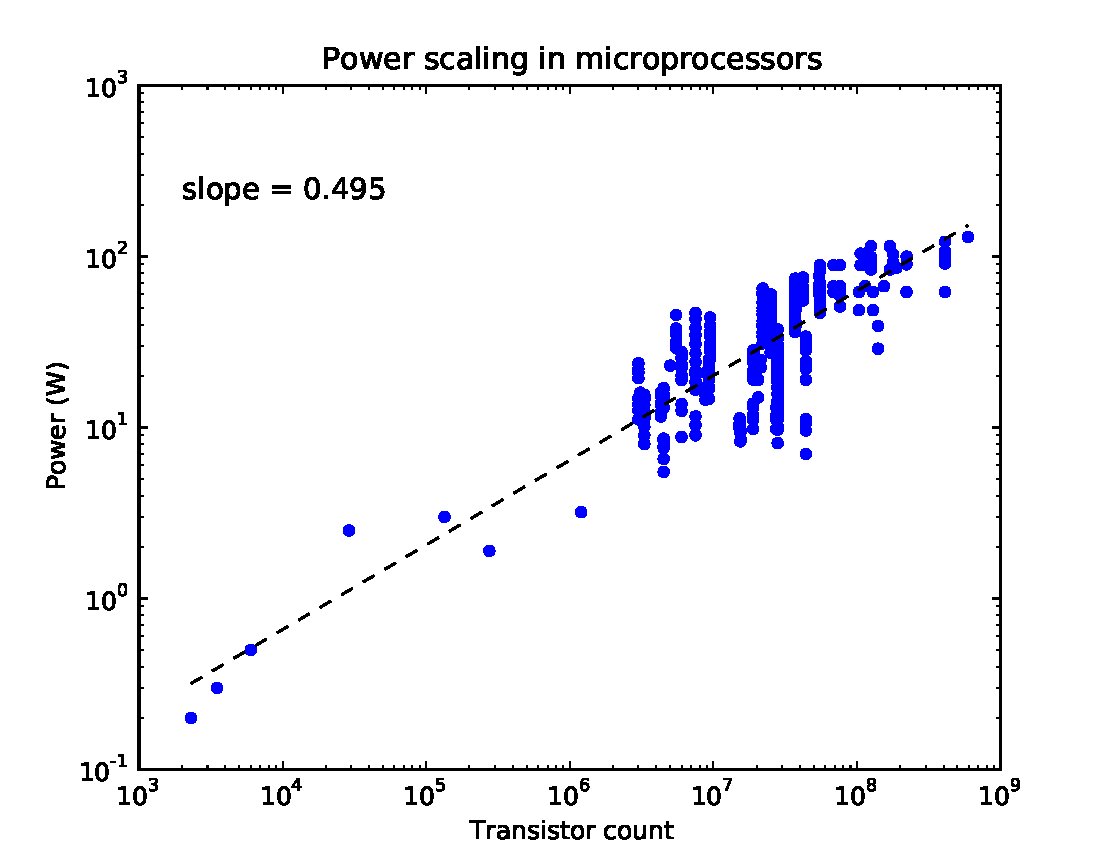
\includegraphics[height=70mm]{Figures/power_scaling.pdf}
\caption{ }
\label{fig:power}
\end{figure}

\begin{figure}[!h]
\centering
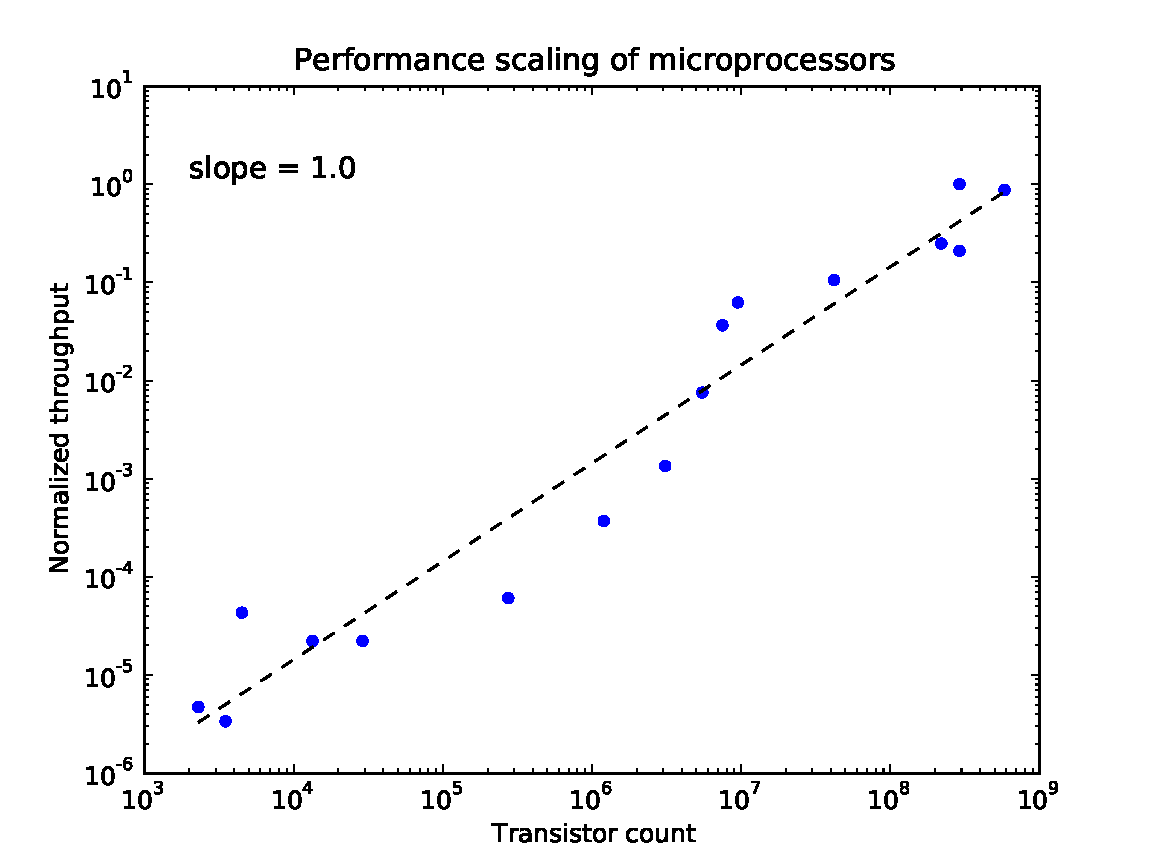
\includegraphics[height=70mm]{Figures/throughput_scaling.pdf}
\caption{ }
\label{fig:throughput}
\end{figure}

Our model provides a simple theoretical explanation for the scaling of 
power and performance in computers over 40 years of microprocessor 
technology improvements.  The excellent agreement between the 
theoretical optimal and experimental data suggests that through 
successive generations of trial-and-error, innovation and 
optimization, engineered designs are highly successful, approaching 
the theoretical limit predicted by the model.

\section{Discussion}

\begin{itemize}
\item By unifying time and energy into a single model, the model
  accounts for the wide variation in size of organisms and computers,
  e.g., mouse to elephant and arm to multe-core.

\item We provide an explanation for Koomey's Law (p. 13)

\item The model shows why computers have given up on reducing clock
  speeds and gone to multi-core.  Once you reach a minimum component
  size, then you are at a transition and a new scaling regime.  What
  is the regime and why is biology the guide?

\item The joule-second as a new fundamental unit of life and
  information.

\item Theoretical explanation for well-known empirical patterns in
  computer architecture.

\item Nature dealt with network design constraints by slowing
  metabolism as animal size increases.  Computer architecture, at
  least until recently, focused on increase clock speeds by minimizing
  component size and incresing energy per chip.  Also, using the third dimension to accommodate more wires, 

\item Computer transions: transistors; transistors to
  integrated circuits; single core to multi-core; desk tops to data centers.
Multicore is an evolutionary transition.  IBM currently making 10 nm chips which are the limit for
  silicon.  IBM recently announced a 7 nm
transistor (more than 1000 times smaller than the diameter of a red
blood cell) and only three times larger than a strand of DNS, using
silicon germanium targeting a 50\% power improvement.  NYT July 9,
2015.  Then going to carbon nanofibers. 

\end{itemize}

\section{Conclusion}

Our analysis provides a unifying explanation for the origin of scaling 
laws in biology and computing. Despite obvious differences in form and 
function, the scaling of organisms and computers is governed by the 
same simple principle.  By minimizing the energy-time product, whether 
through natural selection or engineering, existing designs manage the 
trade-off between cost and performance, leading to general scaling 
patterns observed over several orders of magnitude in size.  Moreover, 
power laws as a function of size are not unique to organisms and 
computers but are widely observed across a large variety of complex 
systems in nature, society and technology.  The scaling of white and 
grey matter in the brain \cite{zhang00}, of energy use and GDP in 
countries \cite{brown11}, and the pace of life and population in 
cities \cite{bettencourt07} are additional examples where a unifying 
explanation is still lacking.  Because cost and performance, i.e., 
energy and time, impose universal constraints, we suggest that a 
common design principle governs the scaling of complex systems that 
process energy, materials and information.

\bibliography{references}
\bibliographystyle{abbrv}

\newpage

\section*{Figure legends}
\paragraph{Figure 1:} Log-log plot of power consumption as a function 
of transistor count for 523 computer microprocessors from different 
vendors and technological generations.  The linear regression slope is 
$0.495$ with correlation coefficient of $0.81$. A regression that 
removes the first seven data points and focuses on the main cloud of 
more modern chips produces a slope of $0.487$.

\paragraph{Figure 2:} Log-log plot of normalized throughput as a 
function of transistor count for 16 Intel microprocessors from 
different technological generations.  The linear regression slope is 
1.0 with correlation coefficient of 0.97.

\end{document}



